\chapter{Fundamentação Teórica}
\label{cap:fundamentacao}

\section{Engenharia de Requisitos}
\label{sec:engenharia_requisitos}

A Engenharia de Requisitos constitui uma das áreas mais relevantes da Engenharia de Software, tendo a responsabilidade de identificar, analisar, declarar, validar e gerenciar as necessidades e expectativas das partes interessadas em relação a um sistema. Seu papel é fundamental desde as fases iniciais do projeto, pois os requisitos estabelecem a base para o planejamento, desenvolvimento e validação do produto de software.

Quando conduzida de forma adequada, ela é responsável por organizar de forma padronizada o escopo do sistema, trazendo benefícios claros ao servir como um instrumento para alinhar as expectativas das partes envolvidas (\textit{stakeholders}) e para guiar a equipe de desenvolvimento na criação do artefato desejado. Além disso, também ajuda a reduzir ambiguidades, retrabalho e falhas de comunicação ao longo do ciclo de desenvolvimento. Em contrapartida, deficiências nessa etapa podem comprometer prazos, custos e a qualidade do artefato construído, estando entre as principais causas de insucesso em projetos de software \cite{sommerville2016}.

Para que o escopo seja definido com precisão, as necessidades do sistema devem ser categorizadas, sendo as principais os Requisitos Funcionais (RF) e os Requisitos Não Funcionais (RNF) \cite{laplante2022}. Essa distinção é fundamental para que o software resultante não apenas apresente as funcionalidades desejadas, mas faça isso enquanto atende a atributos observáveis de qualidade, segurança e usabilidade.

Os Requisitos Funcionais (RF) descrevem os serviços que o sistema deve fornecer, detalhando o que ele deve ser capaz de fazer e como deve reagir às suas entradas \cite{laplante2022}. Um exemplo prático seria ``o sistema deve permitir o cadastro de novos clientes'' ou ``o usuário deve conseguir gerar um relatório de vendas''.

Por outro lado, os Requisitos Não Funcionais (RNF) determinam as restrições e os critérios operacionais que o sistema deve atender, especificando como o software deve se comportar \cite{laplante2022}. Esses requisitos lidam com questões de desempenho, confiabilidade, facilidade de manutenção e restrições de recursos. Na prática, enquanto o requisito funcional define que um relatório deve ser gerado, o não funcional estabelece que a geração deste não pode exceder o tempo de resposta de três segundos, por exemplo.

\subsection{Atividades da Engenharia de Requisitos}

A correta identificação e o gerenciamento desses requisitos funcionais e não funcionais dependem de um ciclo coordenado de atividades, demonstrando que a Engenharia de Requisitos não é um processo único que ocorre somente no planejamento de um projeto, estando presente em todo o ciclo de vida de desenvolvimento de um sistema por meio de atividades iterativas.

Primeiramente, é necessário realizar um levantamento das necessidades e expectativas dos \textit{stakeholders}, o que é feito por meio de técnicas como entrevistas, \textit{workshops}, \textit{brainstorming}, questionários, entre outras \cite{junior2025}. Segundo \citeonline{laplante2022}, essa atividade de Elicitação (ou Descoberta) não é uma simples coleta de dados evidentes, mas um processo investigativo rigoroso. Ele envolve extrair ativamente as necessidades do cliente, descobrir partes interessadas ocultas e determinar os requisitos não funcionais. O resultado desse processo é um conjunto ``cru'' (\textit{raw}) de requisitos iniciais.

Entretanto, a lista inicial de requisitos ``crus'' nem sempre é perfeita. \citeonline{laplante2022} alertam que, logo após serem coletados, esses requisitos frequentemente apresentam problemas: podem ser vagos, incompletos, inconsistentes, interagirem entre si ou apresentarem contradições não óbvias. Isso gera a necessidade de uma etapa de Análise e Acordo. Nessa atividade, ocorre o refinamento da lista inicial, identificando o que realmente é vital para o projeto, eliminando redundâncias e negociando com as partes envolvidas para o alinhamento de expectativas e a resolução de conflitos \cite{junior2025}.

Embora o resultado da análise seja suficientemente consistente, ainda é necessário declará-los de forma padronizada na atividade de Representação (ou Modelagem). Segundo \citeonline{laplante2022}, esta consiste em converter os requisitos processados em modelos para facilitar a comunicação e o posterior desenho da arquitetura. Essa padronização ocorre por meio de três abordagens principais: formais (utilizando uma base matemática rigorosa), informais (com linguagem natural, esboços e diagramas livres) e semiformais (utilizando modelos que podem ser convertidos para representações sólidas) \cite{laplante2022}. A escolha depende da metodologia do projeto, do tamanho da equipe e do nível de precisão exigido. Um exemplo comum, focado na linguagem natural estruturada e utilizado em metodologias ágeis, são as Histórias de Usuário (\textit{User Stories}):

\begin{itemize}
    \item \textbf{Formato padrão:} ``Como um [tipo de usuário], eu quero [ação/funcionalidade] para que [valor/benefício].'' \cite{cohn2004}.
    \item \textbf{Exemplo:} ``Como um cliente cadastrado, eu quero salvar meu cartão de crédito para que minhas futuras compras sejam mais rápidas.''
\end{itemize}

Para que as Histórias de Usuário sejam traduzidas de forma inequívoca para o código, elas raramente operam de forma isolada. Em metodologias ágeis, essa narrativa é complementada por outros elementos essenciais de especificação, notadamente as Regras de Negócio e os Critérios de Aceitação. As Regras de Negócio consistem em diretrizes, políticas ou restrições operacionais que determinam o funcionamento do sistema com base nas normativas da organização (por exemplo, ``o cartão de crédito só pode ser salvo se o usuário tiver autenticação em duas etapas ativada''). Já os Critérios de Aceitação representam as condições claras, objetivas e testáveis que uma funcionalidade específica deve satisfazer para que seja considerada concluída e validada pelo cliente \cite{scrumstudy2024}.

Uma vez elicitadas e padronizadas (com suas respectivas regras e critérios), essas histórias são agrupadas e priorizadas em um artefato central conhecido como \textit{Product Backlog} (ou simplesmente \textit{Backlog}). Este, por sua vez, atua como uma lista dinâmica e ordenada de todas as necessidades, requisitos e melhorias do produto, servindo como a única fonte de verdade sobre o escopo do sistema para a equipe de desenvolvimento \cite{scrumstudy2024}.

Após a representação, é preciso verificar e validar os requisitos. A Verificação garante que a estrutura está correta e completa — por meio de critérios como o INVEST \cite{buglione2013}. A Validação, por sua vez, é o processo de determinar se a especificação é uma representação autêntica das necessidades do cliente, respondendo à pergunta fundamental: ``Estou construindo o produto certo?'' \cite{laplante2022}.

Por fim, para que a lista se mantenha sempre precisa, ocorre o Gerenciamento de Requisitos. Este é um aspecto frequentemente negligenciado, mas vital para lidar com a realidade das mudanças contínuas ao longo do tempo. \citeonline{laplante2022} destacam que o gerenciamento envolve promover a rastreabilidade das alterações e exige que as equipes saibam controlar analiticamente o escopo para evitar o crescimento descontrolado do projeto (\textit{scope creep}).

Toda essa dinâmica de atividades, que vai desde a investigação inicial com as partes interessadas até o controle rigoroso de mudanças em um \textit{backlog}, evidencia a natureza complexa da Engenharia de Requisitos. Consequentemente, o ensino dessa disciplina em uma sala de aula tradicional sofre com dificuldades, pois é um processo que exige vivência, comunicação e resolução de conflitos reais, o que representa um grande desafio para os docentes, tema aprofundado na seção a seguir.

\subsection{Desafios no Ensino}

A elicitação de requisitos, como uma atividade sociotécnica, exige pensamento crítico, comunicação efetiva e tempo considerável para sua realização, esbarrando frequentemente na subjetividade e na dificuldade dos \textit{stakeholders} de articularem o que realmente desejam \cite{sommerville2016, junior2025}. Entretanto, o desenvolvimento das competências relevantes para sua realização apresenta desafios significativos no contexto acadêmico, sendo comum que estudantes em formação apresentem dificuldades em transpor o conhecimento teórico para a prática \cite{lojo2025}.

A abordagem mais eficaz de fomentar tais competências é por meio da prática. Porém, reproduzir as incertezas e ambiguidades de um \textit{stakeholder} real em um ambiente tradicional de sala de aula é um desafio logístico para os docentes \cite{lojo2025}. Além disso, a transição direta para projetos reais traz limitações, pois falhas no levantamento adequado de requisitos podem facilmente levar ao fracasso de um projeto \cite{sommerville2016}, o que tende a gerar insegurança e restringir o espaço seguro para o aprendizado do aluno.

Para contornar tal problema, o uso de simulações apresenta-se como alternativa promissora. Elas promovem a experimentação e o desenvolvimento do raciocínio investigativo em um ambiente prático, com menor exposição aos riscos normalmente presentes em cenários reais. Nesse cenário, ferramentas baseadas em Inteligência Artificial e agentes conversacionais surgem como alternativas promissoras para ampliar oportunidades de prática simulada \cite{ataei2024, schon2026, lojo2025}.

A introdução dessas ferramentas interativas e baseadas em IA para contornar os gargalos do ensino tradicional não deve ser vista como uma iniciativa tecnológica isolada. Pelo contrário, a convergência entre tecnologias digitais avançadas e estratégias de simulação prática materializa a transição rumo a um novo paradigma pedagógico na era digital, amplamente caracterizado na literatura como Educação Inteligente (\textit{Smart Education}), cujos conceitos fundamentais são discutidos a seguir.

\section{Educação Inteligente (\textit{Smart Education})}
\label{sec:educacao_inteligente}

A Educação Inteligente (\textit{Smart Education}) pode ser compreendida como o conceito de aprendizagem na era digital, conforme descrito por \citeonline{zhu2016}. Ela é definida por \citeonline{demir2021} como o uso eficaz e coerente das tecnologias de informação e comunicação (TIC) aliado a abordagens pedagógicas adequadas para atingir resultados de aprendizagem específicos. A essência desse paradigma reside na criação de ambientes inteligentes por meio de tecnologias avançadas, de modo que pedagogias inteligentes possam ser facilitadas para oferecer serviços personalizados e capacitar os alunos \cite{zhu2016}.

A Educação Inteligente se conecta aos conceitos de \textit{e-learning} e \textit{mobile learning} (\textit{m-learning}) como uma etapa evolutiva natural dentro da informática educativa, representando o que \citeonline{demir2021} descreve como a transição dos métodos tradicionais para modelos impulsionados por tecnologias avançadas. Enquanto o \textit{e-learning} foca primordialmente na digitalização e acesso remoto a conteúdos e o \textit{m-learning} enfatiza a mobilidade do aprendiz, a Educação Inteligente integra esses benefícios a uma infraestrutura de computação inteligente, gerando um ecossistema sensível ao contexto e adaptativo, capaz de fornecer suporte personalizado aos estudantes \cite{zhu2016}.

A adoção desse paradigma educacional na sala de aula gera mudanças nos papéis tradicionais dos atores envolvidos no processo de ensino e aprendizagem. Segundo \citeonline{demir2021}, nesse novo cenário, o aluno deixa de ser um receptor passivo para se tornar um indivíduo autônomo, colaborativo e um usuário eficiente de tecnologia. Já o professor, por sua vez, além de guiar o desenvolvimento do estudante, também passa a atuar como suporte tecnológico, auxiliando os alunos no uso das ferramentas digitais e garantindo o pleno aproveitamento do ambiente inteligente.

\subsection{Metodologias Ativas e Simulação Prática}

Metodologias ativas, como a Aprendizagem Baseada em Projetos (PBL - \textit{Project-Based Learning}) e o \textit{Learning by Doing} (aprendizagem pela prática), alinham-se intrinsecamente à implantação da Educação Inteligente. Elas materializam a mudança de papéis na abordagem educativa ao colocar o estudante no centro do processo investigativo \cite{demir2021}, exigindo que ele mobilize conhecimentos teóricos para resolver problemas complexos. No contexto da Engenharia de Software, essas abordagens são fundamentais, pois a absorção passiva de conceitos muitas vezes se mostra insuficiente para preparar o aluno para os desafios dinâmicos do desenvolvimento de sistemas. 

Uma das estratégias mais eficazes para aplicar essa transição no ensino é por meio da adoção de simulações. Essas ferramentas atuam como pontes entre a abstração da sala de aula e a experiência prática que, normalmente, só seria obtida em contextos reais \cite{zhu2016}. Ao reproduzir cenários realistas, incluindo suas incertezas e ambiguidades, os simuladores criam um ambiente seguro para o erro \cite{ataei2024}. Neles, os estudantes podem experimentar livremente a aplicação de seu conhecimento sem as consequências críticas possíveis em um projeto real, promovendo a prática repetida e fomentando a confiança necessária para o pleno desenvolvimento de suas capacidades técnicas. Quando aliadas a tecnologias conversacionais avançadas, como os LLMs, essas simulações viabilizam a prática simultânea e individualizada de turmas inteiras, superando as limitações de escala geradas pela desproporção numérica entre o corpo docente e o volume de alunos \cite{essel2022, soliman2025}. É nesse contexto que o ElicitBot \cite{junior2025} apresenta grande potencial pedagógico.

\section{ElicitBot}
\label{sec:elicitbot}

O ElicitBot, desenvolvido originalmente por \citeonline{junior2025}, é um agente conversacional voltado ao apoio da Engenharia de Requisitos, com ênfase na etapa de elicitação de requisitos funcionais. Tendo como base tecnológica os Modelos de Linguagem de Grande Porte (LLMs), a ferramenta apoia a condução de entrevistas dinâmicas em contextos variados e consolida as informações extraídas, representando os resultados finais em um formato padronizado de Histórias de Usuário (\textit{User Stories}).

Durante a validação dessa prova de conceito, \citeonline{junior2025} constataram a existência de um grande potencial pedagógico na ferramenta. Contudo, tal potencial não pôde ser plenamente explorado devido a limitações inerentes à versão original do sistema. Nesse sentido, o presente trabalho foi concebido com o propósito de viabilizar e potencializar as capacidades educacionais do ElicitBot, mitigando seus gargalos e refinando suas funcionalidades para aplicação em sala de aula.

\subsection{Uso de LLM no ElicitBot}

A atividade de elicitação de requisitos é um domínio complexo, repleto de ambiguidades e informações implícitas. Historicamente, essa complexidade frustrou diversas tentativas de apoiar ou automatizar o processo por meio de sistemas computacionais tradicionais \cite{korn2025, khan2024}. Isso ocorreu devido à incapacidade estrutural dessas ferramentas de lidar adequadamente com a natureza dinâmica dos contextos inerentes a essa etapa. Entretanto, com o surgimento dos Modelos de Linguagem de Grande Porte (LLMs), os sistemas tornaram-se capazes de processar cenários heterogêneos e estruturas semânticas complexas de forma natural, superando a rigidez determinística que limitava as soluções anteriores. Essa flexibilidade, contudo, pode gerar resultados excessivamente genéricos, evidenciando a necessidade de mecanismos capazes de direcionar o comportamento desses modelos para contextos específicos de uso \cite{ataei2024, neumann2025}.

Para materializar esse controle na prova de conceito original, o sistema do ElicitBot foi configurado por meio de um \textit{system prompt} com diretrizes projetadas para orientar o modelo de forma a melhorar seu desempenho na área desejada, evitar alucinações e estabelecer a personalidade a ser emulada pelo modelo: um ``Analista de Requisitos Experiente'' \cite{junior2025}. Durante a simulação (\textit{roleplay}), a ferramenta não atua como uma mera respondente passiva, mas conduz a sessão de elicitação de forma metodológica. As instruções de sistema determinam que a Inteligência Artificial deve fazer perguntas focadas, evitar jargões técnicos para simular um ambiente realista, buscar ativamente o valor de negócio (o ``porquê'' de cada funcionalidade) e pedir esclarecimentos frente a ambiguidades, alinhando-se às boas práticas da literatura da área \cite{sommerville2016}\footnote{A íntegra das instruções de sistema utilizadas na prova de conceito original encontra-se disponível no repositório do projeto em: \url{https://github.com/CedisUnB/ElicitBot-v2/blob/main/docs/prova_de_conceito/system_prompt_poc.md}.}.

Além do diálogo interativo, a arquitetura original operava uma segunda camada estrutural de processamento de linguagem: ao final do fluxo de conversa, um \textit{prompt} de extração analisava o histórico do diálogo para consolidar as informações \cite{khan2024}. Esse processo culminava na geração de um artefato padronizado contendo o requisito principal, as regras de negócio, os critérios de aceitação e uma História de Usuário (US) formatada, fechando o ciclo pedagógico entre a elicitação prática e a documentação formal, conforme proposto por \citeonline{junior2025}\footnote{O detalhamento da padronização original dos requisitos da prova de conceito encontra-se disponível no repositório do projeto em: \url{https://github.com/CedisUnB/ElicitBot-v2/blob/main/docs/prova_de_conceito/prompt_extracao_poc.md}.}.

A Figura \ref{fig:pipeline_llm} ilustra a orquestração paralela desses \textit{prompts} e o fluxo de dados resultante durante a interação do usuário na versão inicial da ferramenta. 

\begin{figure}[htb]
    \centering
    \caption{Fluxograma do Pipeline de Processamento do LLM (Prova de Conceito)}
    \label{fig:pipeline_llm}
    
    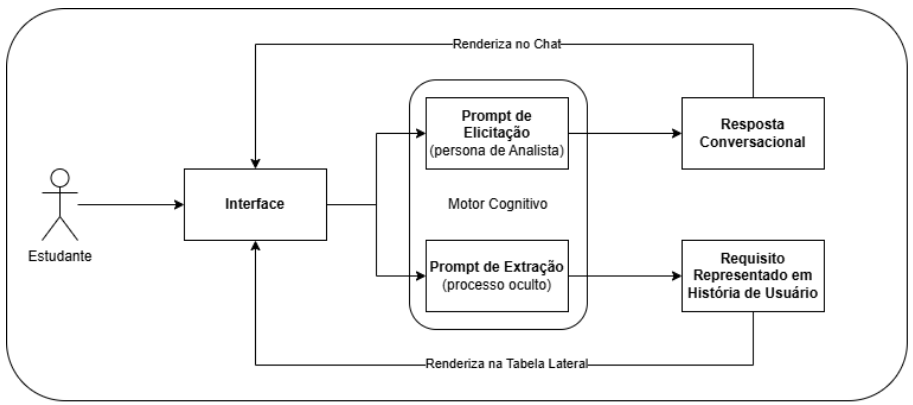
\includegraphics[width=0.9\textwidth]{figuras/pipeline_llm.png}

    \small Fonte: Elaborada pelo autor.
\end{figure}

\subsection{Arquitetura e Funcionamento do Sistema Original}
\label{subsec:arquitetura_poc}

A arquitetura original do ElicitBot foi concebida sob um modelo monolítico e estruturado em camadas, visando garantir a separação de responsabilidades e a facilidade de manutenção inicial \cite{pressman2021, richards2020}. Conforme estabelecido por \citeonline{junior2025}, o sistema organizava-se em três frentes principais: a Interface do Usuário (\textit{Frontend}), o Gerenciamento de LLM (\textit{Backend}) e a Integração com APIs externas. 

O \textit{Frontend} foi implementado utilizando o \textit{framework} Streamlit\footnote{Streamlit. Documentação Oficial. Disponível em: \url{https://docs.streamlit.io/}. Acesso em: 18 jun. 2026.}, que permite a criação de interfaces reativas em Python\footnote{Python. Documentação Oficial. Disponível em: \url{https://www.python.org/doc/}. Acesso em: 18 jun. 2026.}. Para gerenciar a persistência temporária dos dados, a prova de conceito utilizava o mecanismo de \texttt{st.session\_state}, mantendo o histórico de conversa e os artefatos gerados acessíveis apenas enquanto a sessão do usuário estivesse ativa. No núcleo lógico da aplicação (\textit{Backend}), foi adotado o padrão de projeto \textit{Singleton} \cite{gamma1995} na classe \texttt{LLMManager}, garantindo que uma única instância do gerenciador controlasse o estado da interação durante a execução. Além disso, a aplicação utilizava o padrão \textit{Service Layer} \cite{fowler2002}, encapsulando a lógica de comunicação com os modelos de linguagem e isolando-a das regras de interface.

Foram testadas diferentes APIs como motores de processamento, com a versão mais consolidada da prova de conceito utilizando a do Google Gemini Flash. Ela foi configurada para processar as entradas do estudante em tempo real, mantendo a persona de analista experiente, e, ao final da discussão de cada funcionalidade, atuava analisando o diálogo para extrair e consolidar os requisitos funcionais, regras de negócio e critérios de aceitação de forma síncrona.

Quanto à infraestrutura de disponibilização, a implantação do protótipo foi realizada por meio do ambiente \textit{Streamlit Community Cloud}. Essa escolha de hospedagem permitiu a publicação ágil da prova de conceito diretamente a partir do repositório de versionamento (Git\footnote{Git. Documentação Oficial. Disponível em: \url{https://git-scm.com/}. Acesso em: 18 jun. 2026.}), provendo uma infraestrutura gerenciada que garantiu o acesso online necessário para a etapa inicial de validação do projeto original. A Figura \ref{fig:arquitetura_monolitica} ilustra a topologia integrada dessa versão precursora.

\begin{figure}[htb]
    \centering
    \caption{Diagrama de Componentes da Arquitetura Monolítica (As-Is)}
    \label{fig:arquitetura_monolitica}
    
    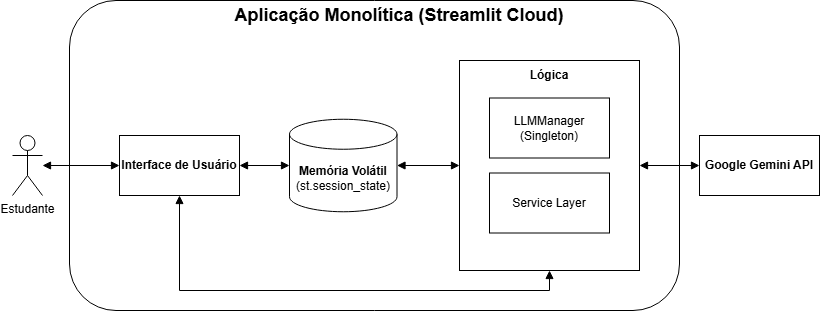
\includegraphics[width=0.9\textwidth]{figuras/arquitetura_monolitica.png}
    
    \small Fonte: Elaborada pelo autor.
\end{figure}

\subsection{Prova de Conceito e Validação Inicial}

A fim de avaliar a eficácia e o potencial pedagógico do ElicitBot, \citeonline{junior2025} conduziram uma etapa de validação prática da prova de conceito com discentes da disciplina de Requisitos de Software da Universidade de Brasília (UnB). Os participantes interagiram com a ferramenta com o intuito de avaliar a usabilidade e a utilidade percebida do sistema. A coleta de dados adotou uma abordagem mista aplicada individualmente, utilizando questionários com escala Likert de 5 pontos e perguntas abertas para diminuir o viés de conformidade social e garantir relatos autênticos.

Os resultados dessa validação indicaram elevada aceitação e percepção positiva de uso da ferramenta. Quantitativamente, o protótipo obteve avaliações elevadas em facilidade de uso, eficiência e clareza das Histórias de Usuário (US) geradas. No âmbito qualitativo, os dados processados por meio de Análise Temática \cite{braun2021} revelaram que os estudantes perceberam a ferramenta como um facilitador cognitivo capaz de auxiliar na estruturação de ideias, na aplicação de conceitos da disciplina e na aceleração do processo de elicitação.

Contudo, a análise também expôs áreas de variação, especialmente na percepção de controle do usuário e na precisão semântica de alguns artefatos gerados. Em conjunto com as limitações da validação, como a possibilidade de vieses de benevolência e de expectativa, o tamanho reduzido da amostra e o domínio simples do projeto testado, esses achados validaram a utilidade da proposta para apoiar o treinamento de iniciantes, mas evidenciaram que o sistema ainda requeria avanços em robustez e flexibilidade interativa para alcançar maior maturidade e consistência pedagógica.

\subsection{Limitações e Oportunidades de Melhoria Previamente Documentadas por Júnior e Oliveira (2025)}

Como desdobramento natural da etapa de validação inicial, o estudo de \citeonline{junior2025} mapeou oportunidades de evolução técnica e funcional para o sistema, servindo como ponto de partida para o diagnóstico conduzido nesta pesquisa. No âmbito da experiência de uso e interação conversacional, os autores apontaram a oportunidade de refinar o controle semântico para reduzir ambiguidades e repetições por parte do agente conversacional. Além disso, identificou-se a necessidade de incorporar mecanismos de controle direto pelo usuário, como edição das respostas e dos artefatos gerados, reinício de etapas e navegação estruturada entre fases da entrevista.

Sob a ótica de infraestrutura e arquitetura de software, a principal restrição de escopo documentada residia no gerenciamento de estado. Como detalhado na Seção \ref{subsec:arquitetura_poc}, a prova de conceito foi dimensionada para validações individuais utilizando a memória temporária da sessão do usuário (\texttt{st.session\_state}). Os próprios autores elencaram a integração de um banco de dados persistente e o desacoplamento da aplicação como trabalhos futuros necessários para preservar o histórico entre sessões e suportar o acesso simultâneo de turmas completas.

Foi precisamente para sanar essas lacunas que o presente trabalho foi estabelecido. Ao diagnosticar o estado herdado da ferramenta, implementar sua reengenharia técnica e funcional e validá-la empiricamente em sala de aula, esta pesquisa buscou consolidar o ElicitBot como uma solução educacional madura, escalável e aplicável de forma controlada no ensino da disciplina de Requisitos de Software.

\section{Trabalhos Correlatos}
\label{sec:trabalhos_correlatos}

Para fundamentar essa evolução e posicionar o ElicitBot diante do estado da arte, torna-se necessário analisar as soluções previamente propostas pela comunidade científica. Nesse contexto, a literatura apresenta diversos estudos sobre o desenvolvimento e/ou aplicação de \textit{chatbots} voltados para as áreas de Engenharia de Software e Engenharia de Requisitos, tanto em contextos educacionais quanto em profissionais. Os trabalhos que se alinham a essa temática foram categorizados e serão discutidos a seguir, iniciando pelo uso de assistentes virtuais no ensino de computação e avançando para aplicações mais específicas na área de requisitos de software.

\subsection{\textit{Chatbots} no Ensino de Computação e Engenharia de Software}

Historicamente, uma das aplicações mais comuns para \textit{chatbots} conversacionais é o suporte informacional e atendimento ao usuário, com alta adoção em setores como o comércio eletrônico, suporte corporativo de TI e triagem de serviços. No contexto acadêmico, essa capacidade de assistência sob demanda tem se mostrado altamente promissora para o apoio ao ensino, assim como demonstra a ferramenta MoodleBot \cite{neumann2025}. Desenvolvida para apoiar o ensino de disciplinas de Ciência da Computação, a solução é capaz de se integrar com o ambiente virtual Moodle para atuar como tutor virtual, esclarecendo dúvidas de estudantes e auxiliando na fixação dos conteúdos teóricos das aulas.

Avançando além do escopo de perguntas e respostas gerais, os modelos de linguagem também vêm sendo explorados no apoio de atividades mais específicas. Esse cenário é ilustrado pelo estudo realizado por \citeonline{nicoletti2025}, que propõe a criação de um \textit{chatbot} integrado com o \textit{framework} Essence. Neste trabalho, a ferramenta atua como suporte na seleção, aplicação e adaptação de práticas de Engenharia de Software focadas na gerência e melhoria de processos de desenvolvimento.

\subsection{\textit{Chatbots} Aplicados à Engenharia de Requisitos}

No âmbito da Engenharia de Requisitos, os \textit{chatbots} também apresentam vasto potencial de aplicação. A etapa de verificação, por exemplo, representa um ponto crítico visto que requisitos mal definidos figuram entre as principais causas de falha em projetos de software. É neste contexto que se insere a ferramenta USQA (\textit{User Story Quality Analyzer}), desenvolvida por \citeonline{jimenez2023}. Baseada em módulos de Processamento de Linguagem Natural (NLP), ela tem o intuito de apoiar estudantes na detecção de anomalias e erros estruturais, avaliar a completude e identificar ambiguidades na criação de Histórias de Usuário.

A popularização dos LLMs ampliou substancialmente as possibilidades de interação na área, impulsionando novas frentes de pesquisa. Aproveitando a capacidade desses modelos de assumir personas e se adaptar a contextos dinâmicos, estudos como os de \citeonline{lojo2025} e \citeonline{schon2026} oferecem aos estudantes a oportunidade de participar de simulações práticas de entrevistas de elicitação. Nessas abordagens, os \textit{chatbots} atuam como \textit{stakeholders}, proporcionando aos alunos experiência prática em um ambiente livre de riscos e aberto à experimentação.

Ao inverter os papéis da ferramenta e do usuário, \citeonline{korn2025} propõem o LLMREI, um modelo conversacional focado na automação do processo de elicitação. O \textit{chatbot} atua como o Engenheiro de Requisitos, conduzindo entrevistas com um \textit{stakeholder} humano nas fases iniciais do projeto para coletar requisitos preliminares. Esses dados podem então ser posteriormente repassados para analistas humanos, viabilizando a condução de entrevistas subsequentes de forma muito mais focada, caso o cenário se prove complexo. Além disso, embora o foco do estudo tenha sido o ganho de escala na elicitação com grandes volumes de \textit{stakeholders}, a ferramenta demonstra aplicações potenciais no treinamento e na educação em Engenharia de Requisitos.

\subsection{Diferenciais deste Trabalho}

A fim de sintetizar o panorama atual das soluções correlatas, a Tabela \ref{tab:trabalhos_correlatos} apresenta um comparativo entre a proposta desta pesquisa e as abordagens identificadas, com ênfase naquelas aplicadas diretamente no contexto da Engenharia de Requisitos. A análise foca no papel desempenhado pela ferramenta, a persona assumida pelo modelo e a capacidade de geração de artefatos padronizados.

{
\footnotesize 
\renewcommand{\arraystretch}{1.1}

\begin{xltabular}{\textwidth}{|p{2.5cm}|X|X|X|p{2cm}|}
    \caption{Comparativo entre Trabalhos Correlatos}
    \label{tab:trabalhos_correlatos} \\
    \toprule
    \textbf{Trabalho} & \textbf{Modo de Atuação} & \textbf{Persona Assumida} & \textbf{Entrega de Requisitos Padronizados} & \textbf{Contexto} \\
    \midrule
    \endfirsthead

    \multicolumn{5}{c}%
    {{\bfseries \tablename\ \thetable{} -- continuação da página anterior}} \\
    \toprule
    \textbf{Trabalho} & \textbf{Modo de Atuação} & \textbf{Persona Assumida} & \textbf{Entrega de Artefatos Padronizados} & \textbf{Contexto} \\
    \midrule
    \endhead

    \midrule \multicolumn{5}{r}{{Continua na próxima página...}} \\
    \endfoot

    \bottomrule
    \multicolumn{5}{c}{\small Fonte: Elaborada pelo autor.} \\
    \endlastfoot
    
    \textbf{ElicitBot (Este trabalho)} & Apoio na elicitação, análise e declaração & Analista de Requisitos Experiente & Sim (artefatos estruturados) & Educacional \\
    \midrule
    LLMREI \cite{korn2025} & Automação de entrevistas preliminares & Analista de Requisitos & Não (Coleta Preliminar) & Industrial \\
    \midrule
    \citeonline{schon2026} & Responde perguntas dos alunos & Cliente / \textit{Stakeholder} & Não (geração feita pelos alunos) & Educacional \\
    \midrule
    \citeonline{lojo2025} & Responde perguntas dos alunos & Cliente / \textit{Stakeholder} & Não (geração feita pelos alunos) & Educacional \\
    \midrule
    USQA \cite{jimenez2023} & Análise estática de artefatos & Revisor & Não (Apenas analisa) & Educacional \\
\end{xltabular}
}

A Tabela \ref{tab:trabalhos_correlatos} demonstra a relevância e a originalidade da abordagem adotada por este trabalho. Ao participar ativamente do processo de elicitação e validação, o ElicitBot diferencia-se do estudo de \citeonline{jimenez2023}; ao assumir o papel de um analista de requisitos, adota uma dinâmica distinta daquelas propostas por \citeonline{schon2026} e \citeonline{lojo2025}, que simulam o cliente. Por fim, sua distinção em relação ao trabalho de \citeonline{korn2025} consolida-se por sua atuação estruturada ao longo de todo o ciclo de descoberta, análise, modelagem relacional de domínio, declaração padronizada e validação de requisitos, somada ao seu direcionamento específico para o contexto acadêmico. Dessa forma, o ElicitBot demonstra capacidade para auxiliar tanto no desenvolvimento do raciocínio crítico necessário para a elicitação quanto na compreensão, por parte do estudante, da estrutura e da rastreabilidade dos artefatos de software. Para materializar esses diferenciais e validar a eficácia da ferramenta em um ambiente real de ensino, adotou-se uma abordagem investigativa aplicada e orientada à construção de artefatos, detalhada no capítulo a seguir.